\documentclass[a4paper,10pt,oneside]{jsbook}
%
\usepackage{amsmath,amssymb,bm}
\usepackage{bm}
\usepackage[dvipdfmx]{graphicx}
\usepackage{ascmac}
\usepackage{makeidx}
\usepackage{txfonts}
\usepackage{indentfirst}
\usepackage{booktabs}
\usepackage{tabularx}
\usepackage{comment}
\AtBeginDvi{\special {pdf:tounicode EUC-UCS2}}
\usepackage[dvipdfmx, setpagesize=false, bookmarks=true, bookmarksnumbered=true]{hyperref}
%
\makeindex
%
\newcommand{\diff}{\mathrm{d}}            %微分記号
\newcommand{\divergence}{\mathrm{div}\,}  %ダイバージェンス
\newcommand{\grad}{\mathrm{grad}\,}       %グラディエント
\newcommand{\rot}{\mathrm{rot}\,}         %ローテーション
%
\setlength{\textwidth}{\fullwidth}
\setlength{\textheight}{44\baselineskip}
\addtolength{\textheight}{\topskip}
\setlength{\voffset}{-0.6in}
%

\begin{document}

%%%%%%%%%%%%%%%%%%%%%%%%%%%%%%%%%%%%%%%%%%%%%%%%%%%%%
% 表紙
\begin{titlepage}
\noindent
国立大学法人 東京大学 生産技術研究所 御中
\begin{center}
	\vspace{8cm}
	{\Huge \textbf{HPC/PFポータルサブシステムGUIの\\機能改修作業} } \\
	\vspace{1cm}
	{\Huge \textbf{作業報告書}} \\
	\vspace{10cm}
	{\Large \textbf{2015年3月20日}} \\
	\vspace{0.5cm}
	{\Large \textbf{株式会社イマジカデジタルスケープ}}
\end{center}
\end{titlepage}

%%%%%%%%%%%%%%%%%%%%%%%%%%%%%%%%%%%%%%%%%%%%%%%%%%%%%
% 目次
\tableofcontents

%%%%%%%%%%%%%%%%%%%%%%%%%%%%%%%%%%%%%%%%%%%%%%%%%%%%%
% 本文
%%%%%%%%%%%%%%%%%%%%%%%%%%%%%%%%%%%%%%%%%%%%%%%%%%%%%
\chapter{はじめに}
本書はHPC/PFポータルサブシステムGUIの機能改修作業の作業報告書である.
2014年12月に開催したセミナー参加者より指摘された操作性に関する要望や,その他の機能向上などを目的として行った改修作業について記述する.

%%%%%%%%%%%%%%%%%%%%%%%%%%%%%%%%%%%%%%%%%%%%%%%%%%%%%
\chapter{GUIの修正に関する作業内容}
GUIの修正に関する作業内容は以下の通りである.

\section{小さなスクリーンでの利用を想定したGUI再デザイン}
通常のノートPCやデスクトップPCにおいてマウス操作を前提とした場合に使い勝手が最適化されるようにGUIの再デザインを行った.
具体的には,ホーム画面,エディット画面において,画面解像度が800x600程度の小さなスクリーンであっても,マウス操作を前提とした閲覧及び編集が可能なGUIデザインに変更した.

\section{プロジェクトエディタ画面上のボタンの整理}
\label{sec:projectbutton}
従来の「RUN」ボタンを廃止し, ワークフローを実行するためのボタンとして「RUN」ボタンを新たに配置した. また. プロジェクトエディタ画面において, ファイルが選択された場合に, 設定ファイルに予め記載している拡張子とアプリケーションの対応関係に基づいて, アプリケーションの起動ボタンが表示されるよう修正を行った.

\section{メイン画面における外部アプリケーション起動ボタンの整理}
メイン画面上の「FXgen」「PDI」ボタンを廃止した. また, \ref{sec:projectbutton} の対応により, プロジェクトエディタ画面において, 対応する拡張子のファイルが選択された際に, 「FXgen」「PDI」などのアプリケーションの起動ボタンが表示されるようになった.

\section{プロジェクトエディタ画面におけるSAVE, STOPボタン押下効果の改善}
プロジェクトエディタ画面のSAVE, STOPボタンに関して, デザインの修正及び押下効果の改善を行った. 
具体的には, SAVEボタン押下時に, 保存されたことを示すポップアップメッセージを表示するように修正を行った.
また, STOPボタンについては, RUNボタンと対の関係であるため, RUNボタン押下時にのみSTOPボタンを表示し, STOPボタンの色を赤く表示することで, 視覚的に分かりやすい動作を実現した.

\section{プロジェクトエディタ画面遷移の検討}
プロジェクトエディタ画面のファイル一覧をツリー表示に変更, ケースを開いた場合においても他のタブウィンドウに遷移せずに元のプロジェクトウィンドウ内で操作が行えるようにした. また, ログ表示, エディット画面, プロジェクト情報画面を, 同一ページ内でボタンによって切り替えられるように修正した. また, 左ペインとエディタ画面との間にセパレータを配置し, 左ペインの幅をセパレータをドラッグすることで可変にする対応を行った.

%%%%%%%%%%%%%%%%%%%%%%%%%%%%%%%%%%%%%%%%%%%%%
\chapter{機能追加に関する作業内容}
機能追加に関する作業内容は以下の通りである.

\section{プロジェクトアーカイブの解凍機能追加}
KDBからダウンロードしたプロジェクトアーカイブをGUI上から選択, 解凍し, プロジェクトとして開く機能を実装した. プロジェクトを開く際のフローは, 図\ref{fig:projectopenflow}のようになる.

\begin{figure}[htbp]
	\begin{center}
		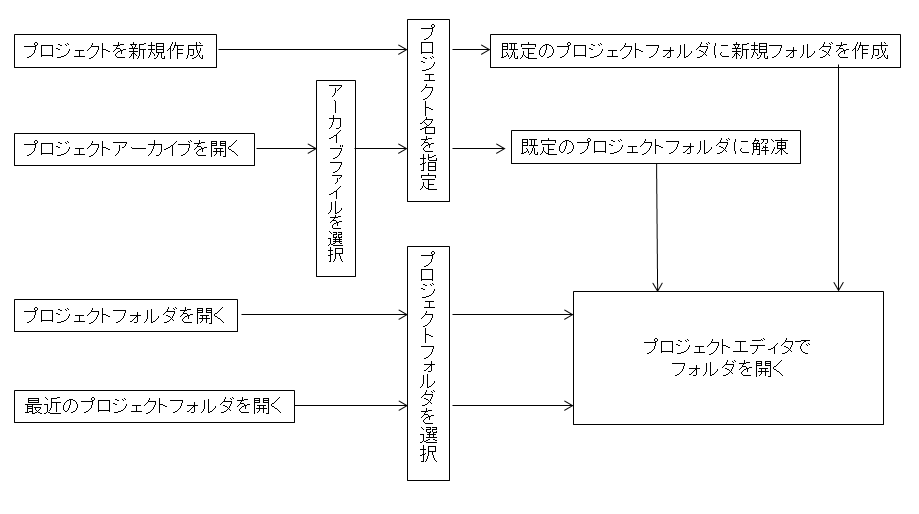
\includegraphics[width=12.0cm]{image/projectopenflow.png}
	\end{center}
	\caption{プロジェクトを開くフロー}
	\label{fig:projectopenflow}
\end{figure}

アーカイブファイルの解凍では, プロジェクトワークフローのファイルpwf.luaがある階層を最上位として, tar.gz圧縮されたファイルに対応している. プロジェクトアーカーブを開くメニューから, tar.gzファイルを選択し, プロジェクト名を指定して開くことで, 既定のプロジェクトフォルダに入力したプロジェクト名で新規にフォルダが作成され, tar.gzファイルが作成されたフォルダ以下に解凍される.

\section{プロジェクトエディタ画面, 及びファイルブラウザ画面におけるファイル一覧の自動更新}
プロジェクトエディタ画面左ペイン及びファイルブラウザ画面において、表示されたフォルダの内容が更新された場合に, それを画面上にも自動反映する仕組みを実装した.

\section{ファイルブラウザ画面転送ファイルの上書き確認及びファイル名変更機能の実装}
ファイルブラウザ画面において, 転送先に同名ファイルが存在した場合に上書き確認する機能を実装した. また, ファイル名を変更する機能を実装した. 

\begin{figure}[htbp]
	\begin{center}
		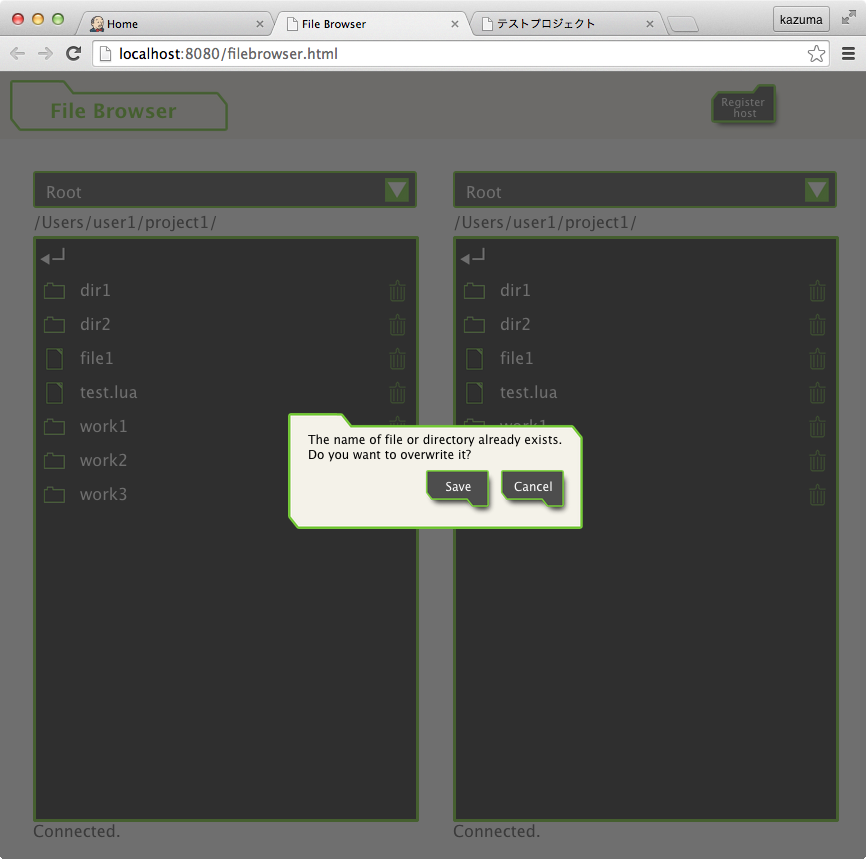
\includegraphics[width=12.0cm]{image/confirm_dialog.png}
	\end{center}
	\caption{上書き確認ダイアログ}
	\label{fig:confirm_dialog}
\end{figure}


\section{リモートジョブ実行時におけるリモートマシン上の作業ディレクトリ自動作成機能の実装}
TODO

%%%%%%%%%%%%%%%%%%%%%%%%%%%%%%%%%%%%%%%%%%%%%
\chapter{データ定義等の設計に関する作業内容}
データ定義等の設計に関する作業内容は以下の通りである.

\section{プロジェクトのメタデータ定義}
TODO

\section{CIFの入出力ファイル情報を利用したワークフロー駆動用APIの設計}
TODO

\section{ワークフローファイルの名称統一}
プロジェクトワークフローのファイル名は, pwf.json, ケースワークフロー名は cwf.luaに統一した.

\end{document}



